% ICASSP 2027 draft using the official 2027 author-kit layout.
\RequirePackage{fix-cm}
\documentclass{article}

\usepackage{spconf,amsmath,amssymb,upgreek,graphicx,booktabs,array,float,placeins,capt-of,enumitem,xcolor}
% Submission PDF: print URLs without active links or PDF bookmarks.
\usepackage{xurl}
\usepackage{microtype}
\usepackage{flushend}

\urlstyle{same}

% Keep large floats with their surrounding discussion and avoid float-only
% pages with excessive vertical whitespace.
\renewcommand{\topfraction}{0.95}
\renewcommand{\dbltopfraction}{0.95}
\renewcommand{\textfraction}{0.05}
\renewcommand{\floatpagefraction}{0.85}
\renewcommand{\dblfloatpagefraction}{0.85}
\setcounter{topnumber}{3}
\setcounter{dbltopnumber}{2}
\setlength{\textfloatsep}{5pt}
\setlength{\dbltextfloatsep}{5pt}
\setlength{\floatsep}{4pt}
\setlength{\dblfloatsep}{4pt}
\setlength{\intextsep}{5pt}
\setlength{\smallskipamount}{1pt}

% ICASSP permits 9-point references. Single-space each entry and leave one
% baseline of extra space between entries, as the linked citation guide asks.
\makeatletter
\let\standardthebibliography\thebibliography
\renewcommand{\thebibliography}[1]{%
  \standardthebibliography{#1}%
  \small
  \setlength{\itemsep}{\baselineskip}%
  \setlength{\parsep}{0pt}%
  \setlength{\parskip}{0pt}%
  \clubpenalty=10000 % Keep a reference's first line with its continuation.
}
% spconf also appends a line break inside \name even though \@maketitle adds
% one itself, leaving an empty row between the names and affiliations.
\renewcommand{\name}[1]{\gdef\@name{{\em #1}}}
% Retain the official template's section and subsection spacing.
\long\def\@makecaption#1#2{%
  \vskip 3pt
  \setbox\@tempboxa\hbox{#1. #2}%
  \ifdim \wd\@tempboxa >\hsize #1. #2\par
  \else \hbox to\hsize{\hfil\box\@tempboxa\hfil}%
  \fi}
\makeatother

\newcommand{\tauvoice}{$\uptau$-Voice}
\newcommand{\taumulti}{$\uptau$-Multilingual}
% Keep revision wrappers visually neutral in the clean manuscript.
\newcommand{\edited}[1]{#1}

\title{TAU-MULTILINGUAL: BENCHMARKING VOICE AGENTS ACROSS LANGUAGES}

\name{{\small Soham Ray$^{1}$\hspace{0.35em}%
Edgard dos Santos Paiva$^{1}$\hspace{0.35em}Ruben Valenzuela$^{1}$\hspace{0.35em}%
Karthik Narasimhan$^{3}$\hspace{0.35em}Keshav Dhandhania$^{1}$\hspace{0.35em}%
Victor Barres$^{2}$}}
\address{{\small $^{1}$Sierra \qquad $^{2}$Mercor \qquad
$^{3}$Princeton University}}

\begin{document}

\maketitle

% Keep the body above ICASSP's 9-point minimum while retaining the official
% heading spacing and four-page technical-content limit.
\fontsize{9.5pt}{11.4pt}\selectfont

\begin{abstract}
English-only benchmarks expose only a narrow slice of voice-agent behavior. We
introduce \taumulti{}, extending \tauvoice{} to Spanish, Brazilian Portuguese,
Hindi, Korean, and Mandarin with native-speaker review and evaluation
of generated language and spoken output. Across 4,500 full-duplex
calls and five voice configurations, Spanish, Portuguese, and Hindi remain
within 3.2 task-completion points of English, but Korean and Mandarin fall by
16.8 and 11.3 points. The failure modes also vary: Korean systems miss more
responses, Mandarin systems interrupt more often, and both struggle with tools
and entities. Grok leads task completion but scores lowest on generation
quality, motivating separate task, interaction, and generation reporting.
We release language packs, validated judges, and tools
for community-built multilingual voice-agent evaluation.
\end{abstract}

\begin{keywords}
multilingual voice agents, spoken dialogue evaluation, task-oriented dialogue,
full-duplex interaction, user simulation
\end{keywords}

\section{Introduction}
\label{sec:introduction}

Voice agents must serve a multilingual world: English is spoken by only 19\% of
the world's population \cite{worldbank2025digital}, yet leading end-to-end voice-agent
benchmarks evaluate English alone
\cite{ray2026tauvoice,bogavelli2026evabench,lin2026fdbv3}.
\edited{Multilingual evaluation must therefore capture task completion, conversational
behavior, linguistic naturalness, and speech fidelity.}

We introduce \taumulti{}, extending \tauvoice{} \cite{ray2026tauvoice} with three
contributions. First, \emph{LanguageFactory} provides a reviewed workflow for
native-speaker-authored simulators, localizing caller personas, speech rules,
and identities while preserving the underlying tasks. Second, we add
human-validated evaluation of linguistic naturalness and speech fidelity
alongside task completion and interaction measures. Third, we evaluate five
voice configurations and two text systems across six languages and three
domains.

\edited{We release the codebase \cite{taumultilingual2026release}
so the community can build callers reflecting local linguistic and cultural
norms, rather than merely translated English personas, alongside
language-specific audits of English-centric agent behavior.}

\begin{figure}[!t]
\centering
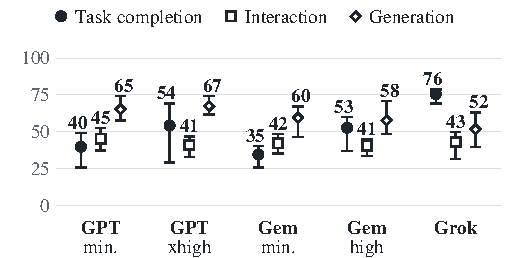
\includegraphics[width=\columnwidth]{figures/model_summary.pdf}
\vspace{-1mm}
\caption{\edited{System means across languages} with worst-to-best language whiskers; \edited{Generation}
excludes English.}
\label{fig:model-summary}
\vspace{\baselineskip}
\captionof{table}{Related benchmarks. A check mark denotes direct evaluation and a
tilde partial coverage. Spk.: spoken; FD: \edited{full-duplex runtime}; Mult.: multilingual;
Int.: \edited{interaction-quality evaluation}; Lang. quality: naturalness and
language use.}
\label{tab:related}
\vspace{4pt}
\centering
\small
\setlength{\tabcolsep}{1.5pt}
\renewcommand{\arraystretch}{0.82}
\begin{tabular*}{\columnwidth}{@{\extracolsep{\fill}}lcccccc@{}}
\toprule
Work & Spk. & FD & Mult. & Task & Int. & Lang. quality \\
\midrule
\multicolumn{7}{l}{\textit{Voice-agent benchmarks}} \\
\tauvoice{} \cite{ray2026tauvoice}
  & $\checkmark$ & $\checkmark$ & -- & $\checkmark$ & $\checkmark$ & -- \\
FDB-v3 \cite{lin2026fdbv3}
  & $\checkmark$ & $\checkmark$ & -- & $\checkmark$ & $\checkmark$ & -- \\
EVA-Bench \cite{bogavelli2026evabench}
  & $\checkmark$ & $\sim$ & -- & $\checkmark$ & $\checkmark$ & $\sim$ \\
M3-DuplexBench \cite{fukuda2026m3duplexbench}
  & $\checkmark$ & $\checkmark$ & $\checkmark$ & -- & $\checkmark$ & -- \\
\addlinespace[2pt]
\multicolumn{7}{l}{\textit{Multilingual speech and dialogue}} \\
VoiceAgentBench \cite{jain2025voiceagentbench}
  & $\checkmark$ & -- & $\checkmark$ & $\sim$ & -- & -- \\
Speech-MASSIVE \cite{lee2024speechmassive}
  & $\checkmark$ & -- & $\checkmark$ & -- & -- & -- \\
X-RiSAWOZ \cite{moradshahi2023xrisawoz}
  & -- & -- & $\checkmark$ & -- & -- & -- \\
GlobalWoZ \cite{ding2022globalwoz}
  & -- & -- & $\checkmark$ & -- & -- & -- \\
\addlinespace[2pt]
\multicolumn{7}{l}{\textit{Language-quality evaluation}} \\
MQM \cite{freitag2021mqm}
  & -- & -- & $\checkmark$ & -- & -- & $\checkmark$ \\
MENLO \cite{whitehouse2026menlo}
  & -- & -- & $\checkmark$ & -- & -- & $\checkmark$ \\
\midrule
\textbf{\taumulti{}}
  & $\checkmark$ & $\checkmark$ & $\checkmark$ & $\checkmark$ & $\checkmark$ & $\checkmark$ \\
\bottomrule
\end{tabular*}
\vspace{3pt}
\end{figure}

\section{Related Work}
\label{sec:related-work}

\tauvoice{} brings the database-grounded tasks of $\uptau$-bench and
$\uptau^2$-Bench \cite{yao2024taubench,barres2025tau2bench} to full-duplex
speech, \edited{evaluating task completion and conversational dynamics but not generation
quality \cite{ray2026tauvoice}. It, EVA-Bench, and FDB-v3 are English-only
\cite{bogavelli2026evabench,lin2026fdbv3}.} M3-DuplexBench covers
English and Japanese turn-taking without executed tool tasks
\cite{fukuda2026m3duplexbench}; VoiceAgentBench evaluates multilingual spoken
tool use at the query/workflow level \cite{jain2025voiceagentbench}; and
Speech-MASSIVE evaluates intent and slot prediction from recorded speech
\cite{lee2024speechmassive}.
X-RiSAWOZ and GlobalWoZ provide multilingual text dialogue with human-verified
or locale-native content \cite{moradshahi2023xrisawoz,ding2022globalwoz}; MQM
and MENLO motivate factorized, human-reviewed language evaluation
\cite{freitag2021mqm,whitehouse2026menlo}. \edited{\taumulti{} combines live voice calls,
tools, environment execution, and naturalness audits
(Table~\ref{tab:related}).}

\section{Methodology}
\label{sec:methods}

\subsection{Matched Multilingual Benchmark}

\edited{\tauvoice{} supplies English task frames, agent policies and tools, user
scenarios, and a simulated caller \cite{ray2026tauvoice}. Its full-duplex
runtime advances in 200-ms ticks; binary rewards check task-specified
environment, action, and communication criteria.} Each
language pack localizes the caller instructions, persona, voice, identity
entities, and evaluation rules while preserving the underlying tasks and
scoring. The same specification drives both voice and matched text conditions,
enabling comparisons by domain, task, system, and reasoning setting.
LanguageFactory stores this specification as a typed, versioned artifact;
Table~\ref{tab:language-factory} illustrates the Hindi pack. Cross-language
differences therefore compare complete localized systems rather than an
isolated causal effect of language.

% Examples are sourced from the released Hindi language pack.
\begin{table}[H]
\caption{LanguageFactory components illustrated with the Hindi pack.
Entity localization maps the same source identity to locale-specific backend
values without changing the task.}
\label{tab:language-factory}
\centering
\small
\setlength{\tabcolsep}{3pt}
\renewcommand{\arraystretch}{0.92}
\begin{tabular}{@{}>{\raggedright\arraybackslash}p{0.28\columnwidth}
                    >{\raggedright\arraybackslash}p{0.65\columnwidth}@{}}
\toprule
Language component & Hindi (India) \\
\midrule
Personas
& Rishika uses fast Hinglish; Imran uses patient, Urdu-inflected Hindi. \\
Speech rules
& Spell with ``R for Rajdhani''; say \emph{at} and \emph{dot} in email
addresses. \\
Task arms and entity localization
& Allison Reeves $\rightarrow$ Neha Gupta; phone: 99400 97181. \\
Audit factors
& Customer address (\emph{aap} vs. \emph{tum/tu}) and agreement with
\emph{aap}. \\
Review and freeze
& Pin the Rishika and Imran voices; freeze preset
\texttt{multilingual\_v1\_hindi}. \\
\bottomrule
\end{tabular}
\end{table}

Native speakers review each pack's language rules, voices, and \edited{pilot calls}.
Automated checks enforce schema, task parity, and persona assignment before
release.

\subsection{Evaluation Cohorts}

\edited{The benchmark contains 900 localized task instances: 50 tasks in each of three
domains, instantiated in six languages. Five voice configurations yield 4,500
primary calls:} GPT (OpenAI \texttt{gpt-realtime-2}) at minimal and xhigh reasoning,
Gemini 3.1 Flash Live Preview at minimal and high, and Grok Voice Think Fast
1.0 \cite{openai2026gptrealtime2,google2026gemini31flashlive,xai2026grokvoicethinkfast}.
\edited{The cascaded caller uses \texttt{gpt-5.5} xhigh for text and Eleven v3 for speech
\cite{openai2026gpt55,elevenlabs2026elevenv3}.} For \edited{task-completion} significance
tests only, the four GPT and Gemini configurations include one additional trial.
We use the short labels GPT, Gemini, and Grok below.

\edited{The matched half-duplex text control evaluates the same 900 localized task
instances with two systems (1,800 calls):} GPT-5.5
xhigh and Gemini 3.1 Pro Preview high
\cite{openai2026gpt55,google2026gemini31pro}. Because both the model and
interaction regime change, this is an end-to-end control rather than a pure
acoustic intervention.

The ablation evaluates the same 30 retail tasks in Hindi and Mandarin with GPT
xhigh and Gemini high. Against the localized, romanized baseline,
\emph{Entity} substitutes source-English identity values, while
\emph{Entity + DB} adds native-script values and matched spell-out, with all
else fixed.

\subsection{Evaluation Measures}

\edited{Task completion} is the \edited{call-level} environment-reward pass rate.
We introduce two complementary quality scores. \emph{Interaction} is a
call-level composite: 100 minus the equal-weight mean of non-response
\edited{(missed/late replies or failure to yield)}, inappropriate interruption
\edited{(talking over the caller)}, selectivity error \edited{(reacting to backchannels, vocal
tics, or non-directed speech)}, \edited{monologues} over 45 seconds, and validated tool
misuse \edited{(incorrect arguments or agent-caused errors)}.
\edited{\emph{Generation quality} (Generation) is the share
of aligned agent utterances passing both linguistic naturalness and speech
fidelity checks.} These composites are
compact representations only; their intermediate values have no calibrated
interpretation. \edited{Naturalness} flags unnatural phrasing.
Speech fidelity uses a multimodal Gemini 3.1 Pro Preview judge
\cite{google2026gemini31pro} to compare each scored agent-audio clip with its
expected text. A severity-$\geq2$ delivery finding or Mandarin tone-induced
meaning flip is a failure. Language-specific diagnostics remain separate.
\edited{English is excluded only from Generation because our Naturalness rubric targets
translationese and native phrasing in the five localized languages.}

\edited{We compare systems within languages and estimate matched performance gaps
relative to English for Task completion and Interaction.}
We do not rank languages: each is a complete localized system, and \edited{naturalness} is
not cross-language calibrated.

\subsection{Human Validation}

\edited{LLM-based judges} enter results only when precision and recall exceed
.75, F1 exceeds .80, and Cohen's $\kappa>.60$. For naturalness and
language-specific diagnostics, labels require consensus from two
native-language annotators. Validation covers tool use, approximately 60
examples per language for naturalness and speech fidelity, and at least 30 per
language-specific diagnostic;
failing measures remain archived.

Separately, reviewers audit 30 completed calls per language, balanced across
domains and systems. They attribute the first
critical error to the agent, simulator, or infrastructure and score eight
caller-quality dimensions---including voice/prosody quality, turn-taking
naturalness, and behavioral plausibility---on a four-point scale \edited{(see the
released audit rubric \cite{taumultilingual2026release})}.

% Declare the double-column float early enough to retain its page-3 placement.
\begin{figure*}[t]
\centering
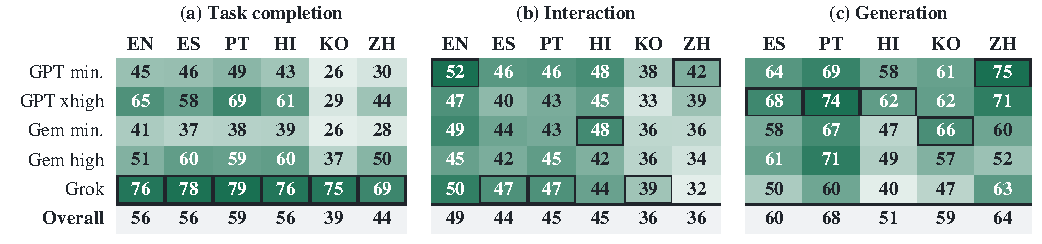
\includegraphics[width=0.98\textwidth]{figures/language_system_heatmaps.pdf}
\caption{\edited{Headline outcomes by system and language. Higher is better; color
scales normalize within panel, outlines mark language-best systems, Overall
averages the five configurations, and Generation excludes English.}}
\label{fig:system-language-heatmaps}
\end{figure*}

\begin{figure}[t]
\centering
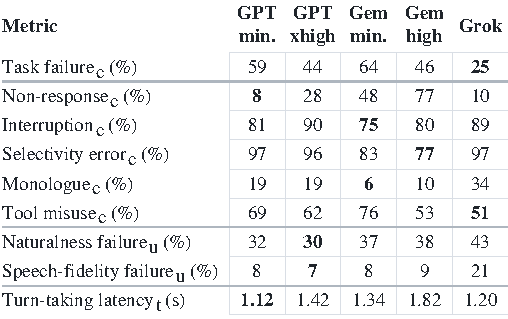
\includegraphics[width=\columnwidth]{figures/model_metric_heatmap.pdf}
\caption{\edited{Main-metric breakdown across languages by system; lower is better.
Bold numbers mark row minima.
Subscripts c/u/r denote call/utterance/response; units are in parentheses.}}
\label{fig:system-diagnostics}
\end{figure}

\subsection{Statistical Analysis}

\edited{Task-completion} inference averages the two trials per task for the four GPT/Gemini
configurations, then compares each language with English across 150 matched
domain--task clusters using paired permutation tests over five contrasts. We
report paired BCa 95\% intervals from 10,000 resamples. Grok
has one trial and appears only in the descriptive estimates in
Figure~\ref{fig:system-language-heatmaps}(a).

Interaction and \edited{Generation} use 100,000 paired cluster-level label-swap
permutations. Interaction compares each language with English after jointly
swapping the five systems and reaggregating component-specific failure and
opportunity counts. \edited{Generation} compares all ten system pairs after jointly
swapping the five localized calls and reaggregating aligned utterances. All
reported confirmatory $p$-values use Holm correction within each family: five
language contrasts for \edited{Task completion} and Interaction, and ten system pairs for
\edited{Generation}. The retail ablations are descriptive.

\section{Results}
\label{sec:results}

\edited{Figures~\ref{fig:system-language-heatmaps} and~\ref{fig:system-diagnostics}
summarize task completion, Interaction, Generation, and their component measures.
We then examine localization failures and model choice.}

\subsection{Task Completion}
\label{sec:results-transfer}

\edited{Task completion} is broadly preserved in Spanish, Portuguese, and Hindi but not in
Korean and Mandarin (Figure~\ref{fig:system-language-heatmaps}(a)). The
confirmatory English-relative losses for Korean and Mandarin are 20.7 and 13.3
points (both Holm-adjusted $p<.00005$); the other three differences are not
significant. The domain pattern is similarly misaligned: telecom is hardest by
\edited{task completion} (44.1\%) yet yields the highest \edited{Generation} (63.2\%).

\edited{The voice--text gap favors pooled text systems in every language by}
16.8--41.5 points. The smallest gap is Spanish; the largest is Korean, where
text reaches 80.3\% versus 38.8\% voice. Because model and turn-taking also
differ, this is an end-to-end voice-system gap rather than a purely acoustic
effect.

\subsection{Interaction}
\label{sec:results-interaction}

Interaction shows the same broad split but a different inferential result: all
five English-relative declines are significant ($p\leq.00055$), with
substantially larger effects for Korean and Mandarin.
The Korean gap concentrates in non-response (46.1\%
versus 27.8\% in English) and tool-use failure (84.9\% versus 49.8\%). Mandarin
instead combines elevated interruption (91.7\% versus 78.0\%) with tool-use
failure (78.8\%). Selectivity failure is high in every language
(86.3--93.5\%), so it is a broad system weakness rather than the main
explanation of the language gap. Spanish and Portuguese show more monologuing
than English, but not the Korean/Mandarin non-response and tool-use pattern.
Similar aggregate Interaction losses thus arise from different operational
failures and imply different remedies.

\subsection{Generation Quality}
\label{sec:results-generation}

\edited{Generation} produces a different model ranking: GPT xhigh leads Spanish,
Portuguese, and Hindi; Gemini minimal leads Korean; and GPT minimal leads
Mandarin (Figure~\ref{fig:system-language-heatmaps}(c)).

\edited{In their naturalness and cultural-grounding audits, native reviewers found
recurring literal or interface-like language:} Spanish
\texttt{user id}, Portuguese ``nenhum voo ainda foi voado'' (no flight has yet
been flown), Hindi ``explicit yes,'' Korean spoken tool names such as
\texttt{check\_sim\_status}, and Mandarin \texttt{toggle data}. Targeted audits
capture different conventions: mixed formal and informal address in Portuguese;
gendered self-reference and omitted \emph{-ji} in Hindi; missing subject
honorification in Korean; and unsuitable titles and missing sentence-final
particles in Mandarin. These diagnostics contextualize \edited{Naturalness} but are not
components of \edited{Generation}. GPT is more natural in Hindi than Gemini and Grok
(35.1--40.6\% versus 49.7--55.5\% failure), yet GPT minimal has the most gender
errors (49.3\%). In Mandarin, GPT has nearly all modal-particle failures
(40.0--59.1\% versus 0--2.0\%).

A related, separate diagnostic is gender agreement. Agent gender was
inadvertently absent from the prompt despite using female voices, yielding
inconsistent self-grounding. Hindi
agents default to masculine self-reference (49.5\% of calls versus 5.3\% with
any feminine form). The overall gender-agreement failure rates---27.2\% in
Hindi and 29.6\% in Portuguese---combine self-reference, noun/anaphora
agreement, and caller-directed errors. Disclosure changes the mix but does not
reliably reduce the total: in 30-call-per-language ablations, failures rise from
30.0\% to 40.0\% in Hindi and fall from 30.7\% to 20.0\% in Portuguese.

\edited{Speech fidelity reveals an all-language provider pattern:} Grok's cleanliness is
79.7\%, versus 91.4--93.9\% for the other systems. Across 71,413 utterances, the
most common material failures are punctuation or formatting errors
(\edited{e.g., speaking punctuation aloud;} 3,529 utterances), mispronunciations (1,362),
and number, date, or currency errors
(1,068).

\subsection{Localization and Entity Handling}
\label{sec:results-localization}

The large Korean and Mandarin task losses concentrate in authentication: exact
lookup succeeds in 81--85\% of English calls, but only 17--55\% of Korean and
37--58\% of Mandarin calls across repeated GPT/Gemini systems. Localized caller
prompts provide the correct family-first name, yet agents often map the spoken
parts into a given-first lookup. In Mandarin, this can break exact lookup even
when callers provide the correct romanized spelling and the agent prompt
requires all tool calls, arguments, and structured outputs in English;
native-character explanations add a separate cross-script mismatch. Telecom's
balanced split shows an exploratory crossover:
Korean task completion is 32.0\% for name+DOB versus 35.2\% for phone
authentication, whereas Mandarin is 40.8\% versus 33.6\%; method remains bundled
with task.

\begin{table}[H]
\caption{Retail entity ablations: task completion (\%) on 30 tasks.}
\label{tab:retail-ablations}
\centering
\small
\setlength{\tabcolsep}{1pt}
\renewcommand{\arraystretch}{0.86}
\begin{tabular*}{\columnwidth}{@{\extracolsep{\fill}}llrrrr@{}}
\toprule
& & \multicolumn{2}{c}{Entity} & \multicolumn{2}{c}{Entity + DB} \\
\cmidrule(lr){3-4}\cmidrule(lr){5-6}
Lang. & System & Localized & Source & Romanized & Native \\
\midrule
Hindi & GPT xhigh & 63.3 & 63.3 & 63.3 & 36.7 \\
 & Gemini high & 60.0 & 66.7 & 60.0 & 60.0 \\
Mandarin & GPT xhigh & 30.0 & 46.7 & 30.0 & 46.7 \\
 & Gemini high & 43.3 & 53.3 & 43.3 & 60.0 \\
\bottomrule
\end{tabular*}
\end{table}

\edited{In the localization ablations, source-English entities match or outperform
localized ones in every cell of}
Table~\ref{tab:retail-ablations}, improving Mandarin by 16.7 points for GPT and
10.0 for Gemini. Replacing romanized database values with native-script names
improves Mandarin by 16.7 points for both systems. Hindi differs: native script
leaves Gemini unchanged and lowers GPT by 26.7 points. These 30-task cells are
\edited{exploratory; exact authentication does not ensure task completion.}

\subsection{Model Choice Across Outcomes}
\label{sec:results-models}

\edited{Figure~\ref{fig:system-diagnostics}} decomposes the model-level tradeoffs.
No configuration dominates; model choice should follow the deployment
objective:
\begin{itemize}[leftmargin=1em,labelsep=.35em,topsep=0pt,partopsep=0pt,
itemsep=1pt,parsep=0pt]
\item \textbf{Task completion:} \edited{Grok leads every language at 75.6\% but has the
lowest Generation (51.8\%).}
\item \textbf{Quality:} GPT xhigh leads \edited{Generation} (67.4\%) \edited{at} 54.4\% \edited{task
completion}; GPT minimal leads Interaction (45.3\%) and has the lowest latency
(1.12 s).
\item \textbf{Stability:} Grok varies least in \edited{task completion}
(9.4-point range), Gemini high in Interaction (11.5), and GPT xhigh in
\edited{Generation} (12.3); Grok varies most in both quality scores.
\item \textbf{Latency:} Higher reasoning raises response latency (GPT:
1.12--1.42 s; Gemini: 1.36--1.82 s). GPT/Gemini calls take 11.3--13.8 min,
versus 25.6 min for Grok.
\end{itemize}

\subsection{Validation and Robustness}
\label{sec:results-validation}

Pooled held-out F1 is 96\% for tool use and 88\% for both naturalness and
speech fidelity; the remaining Interaction components are deterministic.
Among measures \edited{meeting the validation thresholds}, naturalness spans Hindi (F1 81.4\%,
$\kappa=.634$) to Spanish (F1 97.9\%, $\kappa=.965$), and speech fidelity spans
Korean (F1 82.4\%, $\kappa=.754$) to Spanish (F1 96.6\%, $\kappa=.955$).

The separate caller audit also supports the evaluation contract. Reviewers
attribute only 5/180 first critical errors (2.78\%) and 5/104 failed calls
(4.81\%) to the simulator, and none to infrastructure. The eight caller-quality
dimensions average 3.05/4; backchannel naturalness is lowest at 2.86.

Every pair of systems differs significantly on utterance \edited{Generation}; the
weakest contrast is Gemini minimal versus high ($p=.01844$). Interaction effect
sizes preserve the substantive distinction between modest
Spanish/Portuguese/Hindi degradation and large Korean/Mandarin degradation.

\section{Limitations}
\label{sec:limitations}

We study six languages, three domains, three \edited{hosted} model families, and one
speech stack. We did not identify an open-weight model with documented support
for all five localized languages, full-duplex speech, and live tool use.
Evaluation costs limited additional languages, models, and trials.
Simulated callers may not reproduce human timing or repair. \edited{The caller
consumes agent transcripts to minimize simulator-side ASR noise, so synthesis
errors cannot affect task outcomes.} GPT and
Gemini have two trials versus Grok's one; validation sets are finite; and the
voice--text and localization ablations change bundled conditions, so their
effects remain exploratory.

\section{Conclusion}
\label{sec:conclusion}

\taumulti{} shows that multilingual voice-agent reliability extends beyond task
completion. Spanish, Portuguese, and Hindi largely \edited{match English task
completion}, whereas Korean and Mandarin lose ground through authentication,
entity, and interaction failures. Model rankings shift with the objective, so
\edited{joint reporting of task completion, interaction, and generation quality exposes
failures hidden by English-only or outcome-only benchmarks. We release language
packs, validated judges, and tools for community-built multilingual evaluation.}

\FloatBarrier
\raggedcolsend

\section*{\centering\normalsize ACKNOWLEDGMENT}
We thank Ben Shi, Vijay Iyengar, Ola Zytek, and Ajeet Grewal for fruitful
discussions, and Clay Bavor for his continued support.

OpenAI Codex and Anthropic Claude Code assisted with drafting and editing
throughout the manuscript and with developing the benchmark codebase,
analysis code, and figure-generation code, under author review.

\clearpage

\section{Compliance with Ethical Standards}

The benchmark uses no real customer records or recordings. Records are
synthetic and non-sensitive; calls use simulated callers and provider voices.
Reviewers authored benchmark materials and annotated outputs; they consented
and were compensated. Before release, artifacts were screened for incidental
personal data or secrets, and flagged items were excluded.

The benchmark evaluates voice-agent systems, not people or languages; its
results should not be interpreted as measures of human ability or cultural
quality.

This work was supported by Sierra and Mercor. Authors affiliated with Sierra or
Mercor are employees of their respective organizations; the authors have no
other relevant interests to disclose.

\bibliographystyle{IEEEbib}
\bibliography{references}

\end{document}
